\documentclass[authoryearcitations]{UoYCSproject}
\author{Sam Ratcliff}
\title{Quantum Algorithm Synthesis Workbench}
\date{\today}
\supervisor{John A Clark}
\MEng
\wordcount{8832}
\setcounter{tocdepth}{3}
\includes{}

\excludes{}

\abstract{ TO BE DONE
}

\begin{document}
\maketitle
%PUT THESE BACK IN
%\listoffigures
%\listoftables
%\renewcommand*{\lstlistlistingname}{List of Listings}
%\lstlistoflistings
 
\chapter{Introduction}
\chapter{Literature Review}
\section{Introduction to Quantum Computation}
%Historic Introduction
In 1980, Richard Feynmann noted `it is impossible to represent the results of quantum mechanics with a classical universal device`\cite{Feynman82simulatingphysics}.
This statement was a seed for interest in the field of Quantum Computation.
The true power of quantum computation was not initially realised.
The discovery of a quantum algorithm by David Deutsch\cite{Deutsch1985} in 1985 that performed better than a classical computer was the first glimpse of the potential power provided by harnessing quantum mechanics.
However, with slow progress of research into both their implementation and algorithms, the energy behind the research started to decrease.
It would take a discovery by Peter Shor\cite{Shor:1994jg} to reignite the excitement surrounding the subject.  

%What is Quantum Computation
In classical computers the computation is performed using the discrete values of $0$ and $1$.
These values are indicated by +$5$V and $0$V signals propergatating round circuits.
A signal can only be $0$ or $1$, there is no in between value.
Each signal can indicate the value of a single 'bit' of data.
A combination of n bits can be used to represent a number from $0$ to $2^n-1$, an n-bit number.
Classical computation works through the manipulation of these n-bit numbers.


Quantum Computation uses the properties of quantum mechanics to perform computation.
The power of quantum computers come from the use of particles in superpositions.
% This can be seen as the partical being both a $0$ and $1$ simultaneously.
Qubits are the quantum equivalent of the classical bit.
It is these qubits which can be placed into superpositions.
Just as classical computers manipulate bits to perform computation, quantum computers manipulate qubits and their superpositions to perform computation.
The power of these superpositions is not obviously apparent.

It is not possible to observe the superposition of a particle.
When observed the superposition 'collapses' to either logical $0$ or $1$, the basis states.
The probability the the superposition collapses to $0$ is determined by the superposition's properties.

%Explanation of Bra-Ket notation
To write the state of a superposition it is usual to use the 'Bra-Ket' notation, introduced by Dirac\cite{dirac2004principles}.
A 'Ket' is mathematical notation, $\vert$a$\rangle$, which represents a basis function of the respective Hilbert space, $\mathcal{H}$, as a column vector.
\begin{equation}
\vert
a
\rangle = 
\begin{pmatrix}
a_1\\
a_2\\
a_3\\
\vdots
\end{pmatrix}
\end{equation}
Hilbert spaces extend the simple Euclidean vector space into a potential infinite dimension function space.
\begin{figure}
\centering
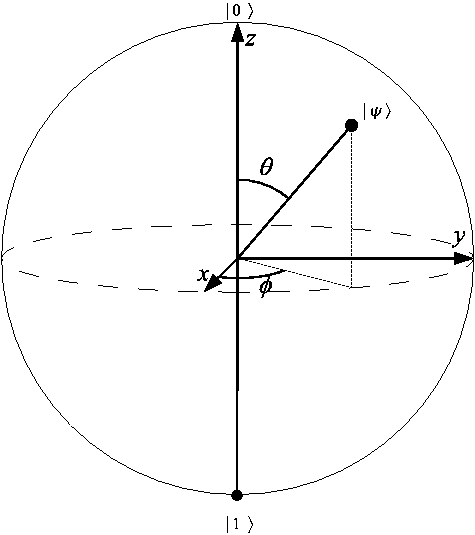
\includegraphics[scale=0.5]{Bloch}
\caption{The 1-Qubit Bloch Sphere \cite{QuantikiBlochSphereImage}}
\label{BlochSphere}
\end{figure}
A quantum state space can also been visualised in terms of the Bloch sphere, shown in Figure \ref{BlochSphere}.
The shown Bloch sphere is for a single qubit system, it can be extended to an n-quibit system however the visualisation breaksdown.
All 'pure' quantum states can be described using the Bloch sphere and all exist on the surface produced by the unit sphere.
In this report only pure quantum states will be used and all explanation of quantum states are more precisely explanations of 'pure' quantum states.
This means that all superpositions of states can be expressed in terms of $|\psi\rangle = \cos \frac{\theta}{2} \, |0 \rangle +  e^{i \phi}  \sin \frac{\theta}{2}  \,|1 \rangle $ with $0 \leq \theta \leq \pi, \quad  0 \leq \phi \leq 2 \pi$, ignoring global phase factors\cite{BlochSphereTalk}.

In quantum mechanics, Kets are used to indicate a state, for example $\vert$0$\rangle$ is the state of a logical $0$ whereas $\vert$1$\rangle$ is the state of logical $1$.
Using this notation and the inclusion of proablities, the state of the superposition can be expressed.

A dual to the Ket notation is the 'Bra' notation, $\langle$a$\vert$.
This notation is used to denote the 'dual vector' of the corresponding ket.
For a state vector represented by
\begin{equation}\label{ket_explanation_example}
\vert
a
\rangle = 
\begin{pmatrix}
a_1\\
a_2\\
a_3\\
\vdots
\end{pmatrix}
\end{equation}
there is a dual vector representing its Hermitian conjugate
\begin{equation}\label{bra_explanation_example}
\langle
a
\vert = 
\begin{pmatrix}
a_1^*$$
a_2^*$$
a_3^*$$
\cdots
\end{pmatrix}
\end{equation}

Combining the two vectors $\langle$a$\vert$ and $\vert$b$\rangle$, written $\langle$a$\vert\vert$b$\rangle$, represents the inner product of the two vectors.
If a and b are unit vectors and $a == b$, $\langle$a$\vert\vert$b$\rangle == 1$.
If a and b are orthogonal, $\langle$a$\vert\vert$b$\rangle == 0$.

The outer product of two vectors, a and b, can be represented by $\vert$a$\rangle$$\langle$b$\vert$.
This represents the transformation from a to b.
It can also be represented in matrix form.

With
$\vert
0
\rangle
== 
\begin {pmatrix}
1\\
0\\
\end{pmatrix}
$
and
$\vert
1
\rangle
==  
\begin {pmatrix}
0\\
1\\
\end{pmatrix}
$
it is possible to represent $1$-qubit operations in the bra-ket notation.
For example, the NOT gate performs a simple negation of a qubit's value.
This can be written as $\vert0\rangle\langle1\vert + \vert1\rangle\langle0\vert$.
Subsituting in the vector values we have
\begin{equation}
\begin{tabular}{ r c l }
\(\begin {pmatrix}
1\\
0
\end{pmatrix}
\begin {pmatrix}
0&&
1
\end{pmatrix}
 + 
\begin {pmatrix}
0\\
1
\end{pmatrix}
\begin {pmatrix}
1&&
0
\end{pmatrix}\)
& \(=\)
& \( 
\begin{pmatrix}
0 && 1 \\
0 && 0
\end{pmatrix}
 + 
\begin{pmatrix}
0 && 0\\
1 && 0
\end{pmatrix}
\) \\
& \(=\)
& \( 
\begin{pmatrix}
0 && 1 \\
1 && 0
\end{pmatrix}
\)
\end{tabular}
\end{equation}

This matrix can be seen as a transformation matrix for the NOT operation.
In quantum computation, the NOT gate is one of the $4$ gates known as the Pauli gates, more specifically the Pauli-X gate.
It is called the Pauli-X gate as it can be seen as a rotation of $\pi$ radians about the X axis of the Bloch sphere, Figure \ref{BlochSphere}.

% Definition of Unitary
The matricies representing the Pauli-X gate and all other quantum logic gates are unitary.
A unitary matrix, U, is one which adheres to
\begin{equation}
U*{\dagger}
U == UU*{\dagger} = I_N
\end{equation}
where $I_N$ is the identity matrix in N dimensions and $U*{\dagger}$ is the complex conjugate of $U$.
% Reversible logic
The implication of all quantum logic operations being unitary is that they are reversible, this is a difference to classical computation.
With many classical logic gates irreversible, there is not a set of quantum logic gates which is as computationally powerful as the set of classical logic gates.
This seems like a major issue, quite the contrary.
The set of classical logic gates can be replaced by reversible equivalents and therefore it is possible to produce a set of quantum logic gates with the equivalent computational power as the classical logic gates.

%Superposition
As with all probablities, the overall probability of a superposition collapsing to any of the states it contains must equal $1$.
\begin{equation}\label{superposition_explanaiton}
\alpha\vert0\rangle+\beta\vert1\rangle
\end{equation}
Equation \eqref{superposition_explanaiton} is how the combination of the logical $0$ and $1$ states in a superposition can be represented for a single particle.
This is equivalent to the representation provided by the Bloch sphere, Figure \ref{BlochSphere}.
The probability of this state collapsing to the basis state $0$ can be calculated by $\vert\alpha\vert^2$ where $\alpha$ is a complex number.
$\alpha$ is known as the probablility amplitude of $\vert0\rangle$.
Similarly, the probability of this state collapsing to the basis state $1$ can be calculated by $\vert\beta\vert^2$, $\beta$ being the probability amplitude of $\vert1\rangle$.
It follows that $\frac{1}{\sqrt{2}}\vert0\rangle+\frac{1}{\sqrt{2}}\vert1\rangle$ is an equal superposition where the collapse to 0 is just as likely as collapsing to $1$.
This provides the first glimpse of where a single qubit has the ability to perform a function not currently possible on a classical computer.
With n-qubits in the equal superposition, we have n binary values which have an equal probability of taking the value $0$ as the value $1$.
With an ordering decided of these qubits, collapsing the superposition of each qubit will result in a binary value of length n.
With all probabilities being $\frac{1}{2}$ this binary value takes a truely random value between $0$ and $2^n-1$.
It is not possible to produce a truely random number using a classical computer.

A second indication of the power held within the idea of superposition becomes clear if we look at the n-qubits in their equal superposition.
In 1935, Erwin Schr$\ddot{o}$ginger proposed a thought experiment to explain the idea of superposition.
Imagine a cat in a fully opaque box with a vile of poison.
The vile may break at any time, a truely random variable.
After sealing the box the state of the cat is not known.
The cat could be alive if the vile has not broken but could just as likely be dead.
Only by looking inside the box will the state of the cat be known.
Until this time the cat could be thought of as both alive and dead at the same time.
If we assign 'dead' to the state $\vert0\rangle$ and 'alive' to the state $\vert1\rangle$ the situation looks very similar to the state we have previously seen.
Therefore, just as the cat can be thought of as both dead and alive at the same time, a qubit in the superposition $\frac{1}{\sqrt{2}}\vert0\rangle+\frac{1}{\sqrt{2}}\vert1\rangle$ can be thought of as both 0 and 1 at the same time.
This leads to a very powerful property of quantum computers.
With n classical bits, a single number in the range 0 to $2^n-1$ can be expressed at any one time.
With n quantum qubits, every number in the range 0 to $2^n-1$ can be expressed at any one time.
This effectively allows computation over the whole range of $2^n$ inputs to be carried out in parallel.

This parallism is very powerful and has been shown to enable the computation of problems classified as NP to be performed in polynomial time.
This does however have a caveat.
As mentioned previously the superposition cannot itself be observed or measured.
When observed the superposition collapses to a basis state with respect to the superposition probability amplitudes.
This means that even though $2^n$ calculations can be performed in parallel, only a single answer can be observed.

% mathematic examples of matracies and the application
Along with the Pauli-X gate, there are an additional 3 Pauli gates.
The Pauli-I gate is the simplest of all quantum gates.
It is the identity gate, the output is identical to the input.
In Dirac notation this is $\vert0\rangle\langle0\vert + \vert1\rangle\langle1\vert$, and in matrix form below
\begin{equation}
\begin{tabular}{ r c l }
\(\begin {pmatrix}
1\\
0
\end{pmatrix}
\begin {pmatrix}
1&&
0
\end{pmatrix}
 + 
\begin {pmatrix}
0\\
1
\end{pmatrix}
\begin {pmatrix}
0&&
1
\end{pmatrix}\)
& \(=\)
& \( 
\begin{pmatrix}
1 && 0 \\
0 && 0
\end{pmatrix}
 + 
\begin{pmatrix}
0 && 0\\
0 && 1
\end{pmatrix}
\) \\
& \(=\)
& \( 
\begin{pmatrix}
1 && 0 \\
0 && 1
\end{pmatrix}
\)
\end{tabular}
\end{equation}

The Pauli-Z gate is similar to the Pauli-X gate, but differs in the axis about which it performs the rotation.
The Pauli-Z gate rotates the quantum state by $\pi$ radians about the Z axis.
This represents a phase flip of the quantum state.
The phase of a state is important when interference is used in computation.
In Dirac notation this is $\vert0\rangle
\langle0\vert + \vert1\rangle(-\langle1\vert$), and in matrix form below
\begin{equation}
\begin{tabular}{ r c l }
\(\begin {pmatrix}
1\\
0
\end{pmatrix}
\begin {pmatrix}
1&&
0
\end{pmatrix}
 + 
\begin {pmatrix}
0\\
1
\end{pmatrix}
\begin {pmatrix}
0&&
-1
\end{pmatrix}\)
& \(=\)
& \( 
\begin{pmatrix}
1 && 0 \\
0 && 0
\end{pmatrix}
 + 
\begin{pmatrix}
0 && 0\\
0 && -1
\end{pmatrix}
\) \\
& \(=\)
& \( 
\begin{pmatrix}
1 && 0 \\
0 && -1
\end{pmatrix}
\)
\end{tabular}
\end{equation}

The Pauli-Y gate is similar to both the Pauli-X and Pauli-Z gates, but differs in the axis about which it performs the rotation.
The Pauli-Y gate rotates the quantum state by $\pi$ radians about the Y axis.
This represents a phase flip followed by a bit flip.
In Dirac notation this is $\vert0\rangle
(i\langle1\vert) + \vert1\rangle(-i\langle0\vert$), and in matrix form below
\begin{equation}
\begin{tabular}{ r c l }
\(\begin {pmatrix}
1 \\
0
\end{pmatrix}
\begin {pmatrix}
0 &&
-i
\end{pmatrix}
 + 
\begin {pmatrix}
0 \\
1
\end{pmatrix}
\begin {pmatrix}
i &&
0
\end{pmatrix}\)
& \(=\)
& \( 
\begin{pmatrix}
0 && -i \\
0 && 0
\end{pmatrix}
 + 
\begin{pmatrix}
0 && 0\\
i && 0
\end{pmatrix}
\) \\
& \(=\)
& \( 
\begin{pmatrix}
0 && -i \\
i && 0
\end{pmatrix}
\)
\end{tabular}
\end{equation}

Along with the single qubit operations, like those above, there are operations which can act over n-qubits.
A simple example of a 2 qubit operation is the controlled-NOT, CNOT, operator.
This is a simple extension of the Pauli-X gate.
\begin{table}
\centering
\begin{tabular}{ l | c || r | }
0 & 0 & 0 \\
0 & 1 & 1 \\
1 & 0 & 1 \\
1 & 1 & 0 \\ \end{tabular}
\caption{Classical CNOT Truth Table}
\label{CNOTTruthTable}
\end{table}
The CNOT gate has a control input which it requies to be in the logical $1$ state for the NOT operation on the second input to be carried out.
In classical logic this would extend the truth table to be as shown in Table \ref{CNOTTruthTable}.
The truth table of the CNOT gate is the same as that of the XOR gate.
The Dirac notaion of the CNOT gate is $\vert00\rangle\langle00\vert + \vert01\rangle\langle01\vert + \vert10\rangle\langle11\vert + \vert11\rangle\langle10\vert$.

\section{An Introduction to Quantum Algorithms}
%Known Quantum Algorithms

Just as with classical computers, the computation to produce the required output given inputs is given in the form of an algorithm.
Quantum algorithms can be constructed in several ways. These definitions are based on those provided by Massey\cite{masseythesis}.

\begin{itemize}
\item A quantum circuit can be used to represent an algorithm at the level of quantum logic gates.
This is similar to a specific purpose circuit diagram for classical systems.
\item A quantum program is a representation of the algorithm in some higher level quantum 'programming' language which would generate the required circuit.
The circuit generated is not defined in this method, just it's behaviour.
This could be seen as slightly more flexible that the quantum circuit model as the 'compiler' can be updated to reflect the findings of future research.
\item A parameterisable quantum algorithm is a representation in pure Psudo-code.
It proves the flexibility of changing some value n, which is used to indicate the number of input qubits, to produce quantum circuits or programs with the desired behaviour on n qubits.
This is the most flexible construction of quantum algorithms.
It can cope with the changing in input size and can use findings of research just like in the 'compliation' of a quantum program.
\end{itemize}

Currently there are very few quantum algorithms known.
Peter Shor has carried out, and published, a discussion on the progress made `in discovering algorithms for computation on a quantum computer`\cite{Shor:2004:PQA:1032132.1032149}.

\subsubsection{Deutsch-Jozsa Algorithm}
%Deutsch-Jozsa Algorithm

\subsubsection{Shor's Factorisation Algorithm}
%Shors Algorithm
In 1994, Peter Shor astonished the computer science community with a factorisation algorithm to run on a quantum computer.
This allowed the factorisation of interger numbers into their consitiuent primes in polynomial time
(READ PAPER) 

\subsubsection{Grover's Search Algorithm}	
%Grovers Database search algorithm
(READ PAPER)

--Problems with current algorithms

	--Scalability
	
	--Require many more Qubits than are available with current hardware implementations


--Current State of QC
	
	--Latest hardware
	
	--Latest algorithms

\section{The Use of Evolutionary Computation in the Synthesis of Quantum Algorithms}
%Need to read a lot more
% different representations
% ways to simulate them

\section{The Focus of this Project}

\bibliography{document}
\end{document}
